\chapter{Анализ секретности системы квантовой коммуникации с недоверенным приемным узлом} \label{ch:ch6}
\section{Исследование возможностей злоумышленника по получению информации о квантовом состоянии при разделении многофотонных состояний} \label{sec:ch6/sec1}

Пусть $|\alpha e^{i \varphi}\rangle$ - слабое когерентное состояниие, где $\alpha$ - это амплитуда состояния, а $\varphi$ - фаза, с помощью которой кодируется бит. Вероятность наблюдения ожидаемого результата измерения, говорящего о наличии $n$ фотонов в данном примере или импульсе, может быть получена с учетом следа продукта матрицы плотности когерентного состояния $\rho$ и проектора на Фоковский базис $|n\rangle\langle n|$: 
%
\begin{align}
    P_n&=\text{Tr}(\rho |n\rangle\langle n|) = \text{Tr}(|\alpha e^{i \varphi}\rangle \langle\alpha e^{i \varphi} |n\rangle\langle n|) \nonumber \\
    &= \text{Tr}(\sum_{k=0}^{\infty}\sum_{m=0}^{\infty} e^{-|\alpha|^2} \frac{(\alpha e^{i \varphi})^k(\alpha^{*} e^{-i \varphi})^m}{\sqrt{k!m!}} |k\rangle\langle m |n\rangle\langle n|) \nonumber  \\
    &=\sum_{j=0}^{\infty}\sum_{k=0}^{\infty}\sum_{m=0}^{\infty} e^{-|\alpha|^2} \frac{(\alpha e^{i \varphi})^k(\alpha^{*} e^{-i \varphi})^m}{\sqrt{k!m!}}\langle j |k\rangle\langle m |n\rangle\langle n|j\rangle \nonumber  \\
    &=e^{-|\alpha|^2} \frac{(|\alpha|^{2n})}{n!}, \label{pnver}
\end{align}
% 
где мы используем свойство ортогональности векторов Фоковского базиса $\langle k| n \rangle = \delta_{kn}$, где $\delta_{kn}$ - дельта-символ Кронекера. Таким образом, мы можем представить слабое когерентное состояние в Фоковском базисе, как:
%
\begin{equation}
    |\alpha e^{i \varphi}\rangle = e^{-\frac{|\alpha|^2}{2}}\sum_{n=0}^{\infty}  \frac{(\alpha e^{i \varphi})^n}{\sqrt{n!}} |n\rangle.
\end{equation}
%
Следовательно, состояние после измерения может быть сокращено следующим образом:
%
\begin{equation}
    \Tilde{\rho}=\frac{\sqrt{|n\rangle\langle n|} |\alpha e^{i \varphi}\rangle \langle\alpha e^{i \varphi} | \sqrt{|n\rangle\langle n|}}{P_n}.
\end{equation}
%
Исследуем, как оператор $\sqrt{|n\rangle\langle n|}$ воздействует на вектор в Фоковском базисе $|m\rangle$, представляя его в виде ряда Тейлора. Рассмотрим два различных случая:
%
\begin{enumerate}
    \item $m \neq n$
    \begin{align}
        \sqrt{|n\rangle\langle n|}|m\rangle = \sum_{k=0}^{\infty} \frac{(-1)^k(2k)!}{(1-2k)(k!)^2 4^k}(|n\rangle\langle n|-\hat{I})^k|m\rangle ,
    \end{align}
    где $\hat{I}$ оператор тождества. Используя следующие свойства
    \begin{gather}
        \hat{I}|m\rangle=|m\rangle, \\
        (|n\rangle\langle n|)^k |m\rangle = (|n\rangle\langle n|)^{k-1} |n\rangle\langle n|m\rangle = 0,
    \end{gather}
    получаем
    \begin{align}
       \sqrt{|n\rangle\langle n|}|m\rangle = \sum_{k=0}^{\infty} \frac{(-1)^k(2k)!}{(1-2k)(k!)^2 4^k}(-1)^k|m\rangle = 0 |m\rangle.
    \end{align}
    \item $m=n$
    
   Затем, используя следующие свойства
    \begin{align}
        (|n\rangle\langle n|)^k |n\rangle = (|n\rangle\langle n|)^{k-1}=\nonumber\\ =|n\rangle\langle n|n\rangle = (|n\rangle\langle n|)^{k-1} |n\rangle = ... = |n\rangle,
    \end{align}
    тогда
    \begin{align}
        \sqrt{|n\rangle\langle n|}|n\rangle &= \sum_{k=0}^{\infty} \frac{(-1)^k(2k)!}{(1-2k)(k!)^2 4^k}(|n\rangle\langle n|-\hat{I})^k|n\rangle \nonumber\\
        &=|n\rangle + \sum_{k=1}^{\infty} \frac{(-1)^k(2k)!}{(1-2k)(k!)^2 4^k}(|n\rangle\langle n|-\hat{I})^k|n\rangle \nonumber\\
        &=|n\rangle + 0 = |n\rangle.
    \end{align}
\end{enumerate}
%
Таким образом, в сокращенном виде:
%
\begin{align}
   \Tilde{\rho}&=\frac{1}{P_n}\sum_{k=0}^{\infty}\sum_{m=0}^{\infty} e^{-|\alpha|^2} \frac{(\alpha e^{i \varphi})^k(\alpha^{*} e^{-i \varphi})^m}{\sqrt{k!m!}} \sqrt{|n\rangle\langle n|}|k\rangle\langle m |\sqrt{|n\rangle\langle n|} \nonumber \\
   &= \frac{1}{P_n} P_n |n\rangle\langle n| = |n\rangle\langle n|. \label{rhored}
\end{align}
%
Тем самым, в соответствии с выражениями, полученными в~\ref{pnver} и \ref{rhored} результат измерения числа фотонов в импульсе (проекция на Фоковский базис) в слабом когерентном импульсе и сокращенное состояние после измерения не содержат информации о фазе когерентного состояния $\varphi$. В случае с множеством мод, проблема сводится к случаю с одной модой, описанному выше.
\pagebreak

%%%%%%%%%%%%%%%%%%%%%%%%%%%%%%%%%%%%%%%%%%%%%%%%%%%%%%%%%%%%%%%%%%%%%%%%%%%%%%%%%
\section{Оценка скорости формирования секретного ключа в асимптотическом приближении} \label{ch:ch6/sec2}

Finally one may derive expression that estimates average sifted key rates $C$ (identical bits but correlated with Eve hence privacy amplification is necessary)
\begin{equation}
    C=FR(1-h(Q)),
\end{equation}
where $h(Q)$ is binary entropy function.

To provide asymptotic key rates we use well-known method introduced by Devetak-Winter \cite{devetak2005distillation}.

We have estimated Holevo information for multi-mode coherent states presented in Eq.~\ref{phi} according to \cite{kozubov2019finite}:
\begin{equation}
    \chi=h\left(\frac{1-e^{-\mu_0(1-d^S_{00}(2\beta))}}{2}\right)\approx h\left(\frac{1-e^{-2\mu}}{2}\right).
\end{equation}
It shows us the maximal amount of information Eve may obtain from the states in one channel. However TF QKD schemes have two independent channels. Hence Eve can perform independent measurements in two quantum channels and obtain the following amount of information:
\begin{equation}
    \tilde{\chi}=2(1-\chi)\chi+\chi^2.
\end{equation}
Thus asymptotic secure key rates $K$ is as follows:
\begin{equation}
     K=FR(1-\xi h(Q)-\tilde{\chi}),
\end{equation}
where $\xi$ is the error correction efficiency. 
For calculations we use experimental parameters from one of the regimes used in Ref.~\cite{Gleim16,Miroshnichenko18}, which are close the implemented during experimental verification of our model: $F=100$ MHz, $\mu=0.1$, $\mu_0=4$, $\Delta\varphi=5^{\circ}$, $\vartheta=10^{-3}$, $\xi=1.15$, $\varphi_0=5^{\circ}$ $\eta_D=0.25$, $\gamma_{dark}= 10$ Hz. The simulation results are shown in Fig.~\ref{fig:fig2}.

\begin{figure}
	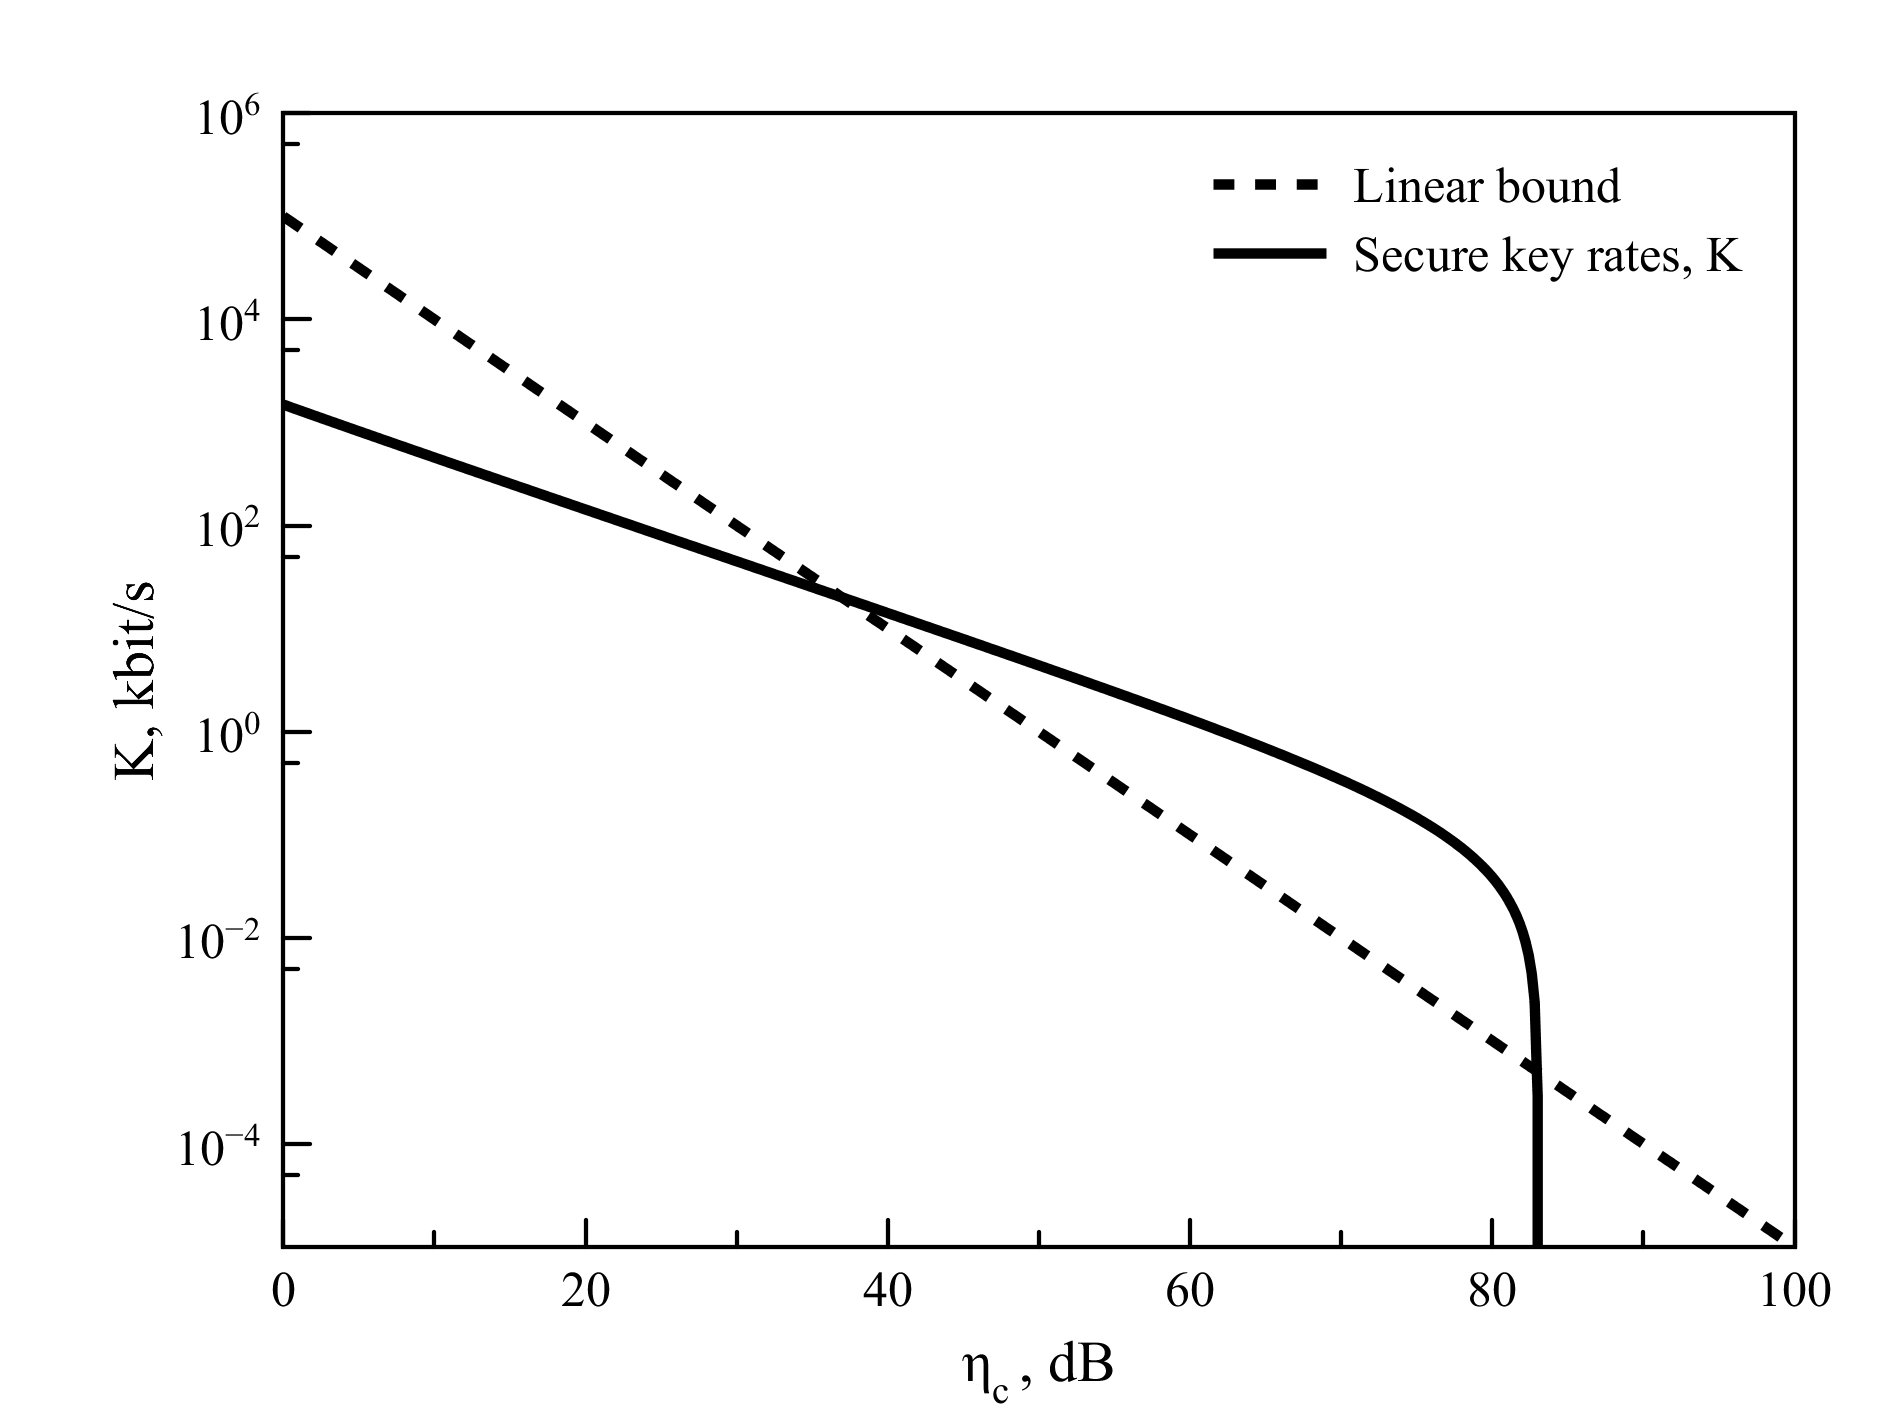
\includegraphics[width=1\linewidth]{TFQKD.png}
	\caption{ Simulation of our TF QKD protocol based on multi-mode phase-coded weak coherent states. For the considered simulation parameters, the key rate of proposed TF QKD exceeds the linear key rate bound by Pirandola et al. (PLOB bound) \cite{pirandola2017fundamental} when $\eta_c \gtrsim$ 40 dB (200 km). In addition, our protocol is also able to achieve a long transmission distance of $\eta_c\approx$ 83 dB (460 km). %Parameters were estimated as follows: $\mu=0.2$, $\mu_0=4$, $F=100$ MHz, $\gamma_{dark}=1.5$ kHz, $\vartheta=10^{-2.5}$, $\varphi_0\approx0$, $\eta=10^{-1.65}$, $\varphi_m\approx3^{\circ}$.} 
	}
	\label{fig:fig2}
\end{figure}


Наконец, можно определить выражение для оценки среднего значения скорости формирования просеянного ключа $K$ (одинаковые биты между легитимными пользователями, но коррелирующие с возможным результатом у злоумышленника, что требует проведения процедуры усиления секретности)
\begin{equation}
    K=FR(1-h(Q)),
\end{equation}
где $h(Q)$ это функция двоичной энтропии. 

\pagebreak

%%%%%%%%%%%%%%%%%%%%%%%%%%%%%%%%%%%%%%%%%%%%%%%%%%%%%%%%%%%%%%%%%%%%%%%%%%%%%%%%%%
\section{Выводы по главе} \label{ch:ch6/sec9}


В \ref{ch:ch6/sec2}  

\pagebreak

\chapter{Оформление различных элементов} \label{ch:ch10}

\section{Форматирование текста} \label{sec:ch10/sec1}

Мы можем сделать \textbf{жирный текст} и \textit{курсив}.

\section{Ссылки} \label{sec:ch10/sec2}
Сошлёмся на библиографию.
Одна ссылка: \cite[с.~54]{Sokolov}\cite[с.~36]{Gaidaenko}.
Две ссылки: \cite{Sokolov,Gaidaenko}.
Много ссылок: %\cite[с.~54]{Lermontov,Management,Borozda} % такой «фокус»
%вызывает biblatex warning относительно опции sortcites, потому что неясно, к
%какому источнику относится уточнение о страницах, а bibtex об этой проблеме
%даже не предупреждает
\cite{Lermontov, Management, Borozda, Marketing, Constitution, FamilyCode,
Gost.7.0.53, Razumovski, Lagkueva, Pokrovski, Methodology, Nasirova, Berestova,
Kriger}%
\ifnumequal{\value{bibliosel}}{0}{% Примеры для bibtex8
    \cite{Sirotko, Lukina, Encyclopedia}%
}{% Примеры для biblatex через движок biber
    \cite{Sirotko2, Lukina2, Encyclopedia2}%
}%
.
И~ещё немного ссылок:
\cite{Article,Book,Booklet,Conference,Inbook,Incollection,Manual,Mastersthesis,
Misc,Phdthesis,Proceedings,Techreport,Unpublished}
% Следует обратить внимание, что пробел после запятой внутри \cite{}
% обрабатывается ожидаемо, а пробел перед запятой, может вызывать проблемы при
% обработке ссылок.
\cite{medvedev2006jelektronnye, CEAT:CEAT581, doi:10.1080/01932691.2010.513279,
Gosele1999161,Li2007StressAnalysis, Shoji199895, test:eisner-sample,
test:eisner-sample-shorted, AB_patent_Pomerantz_1968, iofis_patent1960}
\ifnumequal{\value{bibliosel}}{0}{% Примеры для bibtex8
}{% Примеры для biblatex через движок biber
    \cite{patent2h, patent3h, patent2}%
}%
.

\ifnumequal{\value{bibliosel}}{0}{% Примеры для bibtex8
Попытка реализовать несколько ссылок на конкретные страницы
для \texttt{bibtex} реализации библиографии:
[\citenum{Sokolov}, с.~54; \citenum{Gaidaenko}, с.~36].
}{% Примеры для biblatex через движок biber
Несколько источников (мультицитата):
% Тут специально написано по-разному тире, для демонстрации, что
% применение специальных тире в настоящий момент в biblatex приводит к непоказу
% "с.".
\cites[vii--x, 5, 7]{Sokolov}[v"--~x, 25, 526]{Gaidaenko}[vii--x, 5, 7]{Techreport},
работает только в \texttt{biblatex} реализации библиографии.
}%

Ссылки на собственные работы:~\cite{vakbib1, confbib1}

Сошлёмся на приложения: Приложение \ref{app:A}, Приложение \ref{app:B2}.

Сошлёмся на формулу: формула \eqref{eq:equation1}.

Сошлёмся на изображение: рисунок \ref{fig:knuth}.

Стандартной практикой является добавление к ссылкам префикса, характеризующего тип элемента.
Это не является строгим требованием, но позволяет лучше ориентироваться в документах большого размера.
Например, для ссылок на рисунки используется префикс \textit{fig},
для ссылки на таблицу -- \textit{tab}.

В таблице \ref{tab:tab_pref} приложения \ref{app:B4} приведён список рекомендуемых
к использованию стандартных префиксов.

\section{Формулы} \label{sec:ch6/sec3}

Благодаря пакету \textit{icomma}, \LaTeX~одинаково хорошо воспринимает
в~качестве десятичного разделителя и запятую ($3,1415$), и точку ($3.1415$).

\subsection{Ненумерованные одиночные формулы} \label{subsec:ch10/sec3/sub1}

Вот так может выглядеть формула, которую необходимо вставить в~строку
по~тексту: $x \approx \sin x$ при $x \to 0$.

А вот так выглядит ненумерованая отдельностоящая формула c подстрочными
и надстрочными индексами:
\[
(x_1+x_2)^2 = x_1^2 + 2 x_1 x_2 + x_2^2
\]

При использовании дробей формулы могут получаться очень высокие:
\[
  \frac{3}{\sqrt{2}+
  \displaystyle\frac{1}{\sqrt{2}+
  \displaystyle\frac{1}{\sqrt{2}+\cdots}}}
\]

В формулах можно использовать греческие буквы:
\[
\alpha\beta\gamma\delta\epsilon\varepsilon\zeta\eta\theta\vartheta\iota\kappa%
\lambda\\mu\nu\xi\pi\varpi\rho\varrho\sigma\varsigma\tau\upsilon\phi\varphi%
\chi\psi\omega\Gamma\Delta\Theta\Lambda\Xi\Pi\Sigma\Upsilon\Phi\Psi\Omega
\]

Для красивых дробей (например, в индексах) в
\verb+userstyles.tex+ диссертации добавлен макрос
\verb+\slantfrac+, благодаря которому можно
писать $\slantfrac{1}{2}$ вместо $1/2$.

\subsection{Ненумерованные многострочные формулы} \label{subsec:ch10/sec3/sub2}

Вот так можно написать две формулы, не нумеруя их, чтобы знаки <<равно>> были
строго друг под другом:
\begin{align}
  f_W & =  \min \left( 1, \max \left( 0, \frac{W_{soil} / W_{max}}{W_{crit}} \right)  \right), \nonumber \\
  f_T & =  \min \left( 1, \max \left( 0, \frac{T_s / T_{melt}}{T_{crit}} \right)  \right), \nonumber
\end{align}

Выровнять систему ещё и по переменной $ x $ можно, используя окружение
\verb|alignedat| из пакета \verb|amsmath|. Вот так:
\[
    |x| = \left\{
    \begin{alignedat}{2}
        &&x, \quad &\text{eсли } x\geqslant 0 \\
        &-&x, \quad & \text{eсли } x<0
    \end{alignedat}
    \right.
\]
Здесь первый амперсанд (в исходном \LaTeX\ описании формулы) означает
выравнивание по~левому краю, второй "--- по~$ x $, а~третий "--- по~слову
<<если>>. Команда \verb|\quad| делает большой горизонтальный пробел.

Ещё вариант:
\[
    |x|=
    \begin{cases}
    \phantom{-}x, \text{если } x \geqslant 0 \\
    -x, \text{если } x>0
    \end{cases}
\]

Кроме того, для  нумерованых формул \verb|alignedat| делает вертикальное
выравнивание номера формулы по центру формулы. Например, выравнивание
компонент вектора:
\begin{equation}
 \label{eq:2p3}
 \begin{alignedat}{2}
{\mathbf{N}}_{o1n}^{(j)} = \,{\sin} \phi\,n\!\left(n+1\right)
         {\sin}\theta\,
         \pi_n\!\left({\cos} \theta\right)
         \frac{
               z_n^{(j)}\!\left( \rho \right)
              }{\rho}\,
           &{\boldsymbol{\hat{\mathrm e}}}_{r}\,+   \\
+\,
{\sin} \phi\,
         \tau_n\!\left({\cos} \theta\right)
         \frac{
            \left[\rho z_n^{(j)}\!\left( \rho \right)\right]^{\prime}
              }{\rho}\,
            &{\boldsymbol{\hat{\mathrm e}}}_{\theta}\,+   \\
+\,
{\cos} \phi\,
         \pi_n\!\left({\cos} \theta\right)
         \frac{
            \left[\rho z_n^{(j)}\!\left( \rho \right)\right]^{\prime}
              }{\rho}\,
            &{\boldsymbol{\hat{\mathrm e}}}_{\phi}\:.
\end{alignedat}
\end{equation}

Ещё об отступах. Иногда для лучшей <<читаемости>> формул полезно
немного исправить стандартные интервалы \LaTeX\ с учётом логической
структуры самой формулы. Например в формуле~\ref{eq:2p3} добавлен
небольшой отступ \verb+\,+ между основными сомножителями, ниже
результат применения всех вариантов отступа:
\begin{align*}
\backslash! &\quad f(x) = x^2\! +3x\! +2 \\
  \mbox{по-умолчанию} &\quad f(x) = x^2+3x+2 \\
\backslash, &\quad f(x) = x^2\, +3x\, +2 \\
\backslash{:} &\quad f(x) = x^2\: +3x\: +2 \\
\backslash; &\quad f(x) = x^2\; +3x\; +2 \\
\backslash \mbox{space} &\quad f(x) = x^2\ +3x\ +2 \\
\backslash \mbox{quad} &\quad f(x) = x^2\quad +3x\quad +2 \\
\backslash \mbox{qquad} &\quad f(x) = x^2\qquad +3x\qquad +2
\end{align*}

Можно использовать разные математические алфавиты:
\begin{align}
\mathcal{ABCDEFGHIJKLMNOPQRSTUVWXYZ} \nonumber \\
\mathfrak{ABCDEFGHIJKLMNOPQRSTUVWXYZ} \nonumber \\
\mathbb{ABCDEFGHIJKLMNOPQRSTUVWXYZ} \nonumber
\end{align}

Посмотрим на систему уравнений на примере аттрактора Лоренца:

\[
\left\{
  \begin{array}{rl}
    \dot x = & \sigma (y-x) \\
    \dot y = & x (r - z) - y \\
    \dot z = & xy - bz
  \end{array}
\right.
\]

А для вёрстки матриц удобно использовать многоточия:
\[
\left(
  \begin{array}{ccc}
    a_{11} & \ldots & a_{1n} \\
    \vdots & \ddots & \vdots \\
    a_{n1} & \ldots & a_{nn} \\
  \end{array}
\right)
\]

\subsection{Нумерованные формулы} \label{subsec:ch10/sec3/sub3}

А вот так пишется нумерованая формула:
\begin{equation}
  \label{eq:equation1}
  e = \lim_{n \to \infty} \left( 1+\frac{1}{n} \right) ^n
\end{equation}

Нумерованых формул может быть несколько:
\begin{equation}
  \label{eq:equation2}
  \lim_{n \to \infty} \sum_{k=1}^n \frac{1}{k^2} = \frac{\pi^2}{6}
\end{equation}

Впоследствии на формулы (\ref{eq:equation1}) и (\ref{eq:equation2}) можно ссылаться.

Сделать так, чтобы номер формулы стоял напротив средней строки, можно,
используя окружение \verb|multlined| (пакет \verb|mathtools|) вместо
\verb|multline| внутри окружения \verb|equation|. Вот так:
\begin{equation} % \tag{S} % tag - вписывает свой текст
  \label{eq:equation3}
    \begin{multlined}
        1+ 2+3+4+5+6+7+\dots + \\
        + 50+51+52+53+54+55+56+57 + \dots + \\
        + 96+97+98+99+100=5050
    \end{multlined}
\end{equation}

Используя команду \verb|\labelcref| из пакета \verb|cleveref|, можно
красиво ссылаться сразу на несколько формул
(\labelcref{eq:equation1,eq:equation3,eq:equation2}), даже перепутав
порядок ссылок \verb|(\labelcref{eq:equation1,eq:equation3,eq:equation2})|.
